\section{Epipolar Geometrie}
\label{sec:epipolar} 

Kurze zusammenfassung bis hier her..
%\textcolor{red}{Epipolar geometry is central to stereovision. On the one hand, knowing
%	it enables to strongly constrain the problem of matching two images.
%	On the other hand, it can be estimated from matches and then allows
%	for motion estimation, self-calibration, and triangulation of 3D points
%	or other geometric primitives.\cite{CamerModels.}}

Die Epipolargeometrie beschreibt ähnlich der Homographie eine Beziehung der projektiven Geometrie zwischen zwei Bildern\cite{HZ}. Sie dient insbesondere zur Korrespondenzanalyse von Punkten aus Bildern und zur Gewinnung von 3D-Informationen die abgebildete Szene. Im Gegensatz zur Homographie ist die Epipolargeometrie unabhängig vom Szenenaufbau, sondern hängt nur von den intrinsischen Parametern der Kamera, sowie deren relative Position zueinander ab.\cite{HZ}. Ohne Kenntnis der Kamerapositionen, kann mit Hilfe der Epipolargeometrie überprüft werden, ob eine Korrespondenz zwischen den Bildpunkten zweier Bilder besteht. Unter korrespondierenden Punkten versteht man Bildpunkte auf zwei Bildern, die Abbilder des selben Objektpunktes im 3D-Raum sind. Ein Beispiel für korrespondierende Punkte wären die Punkte Bildpunkte $m_\tau$ und $m_\tau'$. Diese entstanden aus der Projektion von $M_\delta$ auf zwei Bildebenen mit $m_\tau = PM_\delta$ und $m'_{\tau'} = P'M_\delta$. Die Verbindungsvektoren zwischen den Projektionszentren $C$ und $C'$ mit dem 3D-Objektpunkt $M_\delta$ und die Basislinie, welche die Projektionszentren verbidnet, bilden die Epipolarebene. Auf Abbildung \ref{fig:Epipolargeometry} ist sie als Dreieck zwischen den Punkten zu sehen. Die Epipolargeometrie beschreibt in die Beziehung zwischen den durch Schnitt der Bildebenen und der Epipolarebene entstehenden Schnittgeraden. Für jeden Objektpunkt im Raum, entsteht eine neue solche Ebene, die alle die Basislinie als Drehachse besitzen\cite{HZ}. Dementsprechend entstehen pro neuen Opbjektpunkt im Raum auch jeweils zwei Schnittgeraden. Die Schnittgeraden werden als Epipolarlinien $l$ und $l'$ bezeichnet. $l'$ wird als die zu zum Bildpunkt $m_\tau$ korrespondierende Epipolarlinie bezeichnet und $l$ die zum Bildpunkt $m'_{\tau'}$ korrespondierende Epipolarlinie.  Die Epipolarlinien eines Bildes verlaufen alle durch einen Epipol $e$ oder $e'$ und den abgebildeten Bildpunkten und bilden somit,auf den jeweiligen Bildebenen, ein Bündel aus Epipolarlinien. Epipol $e$ ist die Abbildung von $C'$ auf der Bildebene $I$ von $C$ und Epipol $e'$ ist die Abbildung von $C$ auf Bildebene $I'$ von $C'$. Die Schnittpunkte der Basislinie mit den Bildebenen ergeben die jeweiligen Epipole. Ist eine der Bildebenen parallel zur Basislinie ausgerichtet, so kommt es zu keinem Schnittpunkt der Basislinie mit der parallelen Bildebene und der Epipol befindet sich somit im unendlichen\cite{HZ,ZZGXr}.

\begin{minipage}{\linewidth}
	\centering
	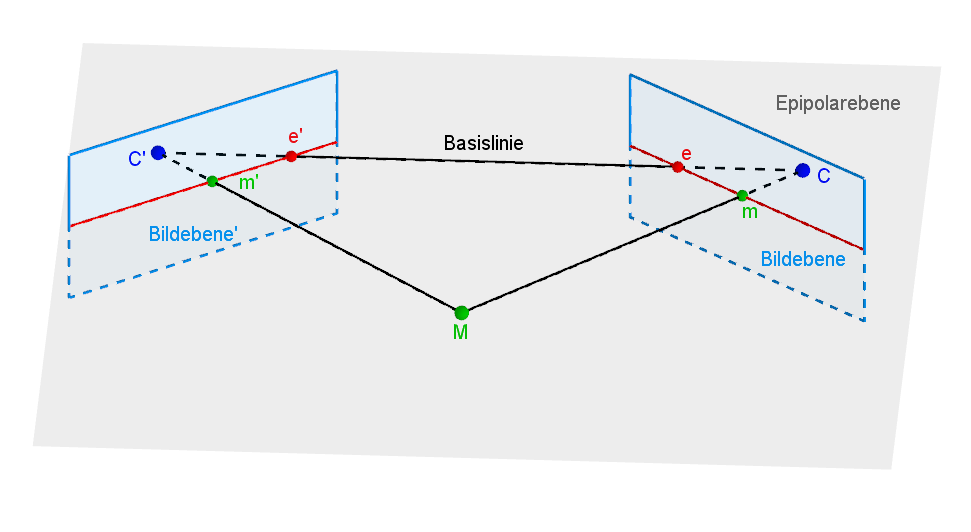
\includegraphics[width=.8\linewidth]{images/EpipolarGeoemtrieGrafik.png}
	\captionof{figure}{$C$ und $C'$ sind die Projektionszentren zweier Kameras. Beide Kameras besitzen jeweils eine Bildebene. Die Basislinien verbindet die Projektionszentren der Kameras. Der Punkt an welchem die Basislinie die Bildebenen schneidet, wird als Epipol bezeichnet. Durch den Epipol verlaufen alle Epipolarlinien des Bildes. $M$ ist der Objektpunkt im 3D-Raum und $m_1$ und $m_2$ sind die jeweiligen Abbildungen dieses Punktes auf den Bildebenen. Die Verbindungsvektoren zwischen $C, C'$ und $M$ bilden die sogenannte Epipolarebene\cite{Elements,HZ,ZZGXr}.}  
	\label{fig:Epipolargeometry}
\end{minipage}\\ \\

Ein Objektpunkt $M_\delta$ wird auf die Bildebenen $I$ und $I'$ der beiden Kameras $C$ und $C'$ projiziert. Es entstehen die zueinander korrespondierenden Bildpunkte $m_\tau$ und $m'_{\tau'}$. Die durch die Bildpunkte $m_\tau$ und $m'_{\tau}$ und den entsprechenden Epipolen $e$ und $e'$ verlaufenden Epipolarlinien, sind zueinander korrespondierende Epipolarlinien. Die zum Punkt $m_\tau$ korrespondierende Epipolarlinie $l'$ beinhaltet alle zu $m_\tau$ möglichen korrespondierenden Punkte, darunter eben auch der eindeutig korrespondierende Punkt $m'_{\tau'}$. Die Epipolargeometrie beschreibt weiterhin eine Beziehung zwischen einem Bildpunkt $m$ und dessen korrespondierender Epipolarlinie $l'$. Diese Beziehung ist der sogenannte ist der sogenannte \textit{Epipolar-Constraint}\cite{HZ,Zhang2014,ZZGXr}. Abbildung \ref{fig:Epipolarconstraint} veranschaulicht die soeben genannte Beziehung eines Bildpunktes zu seiner korrespondierenden Epipolarlinie noch mal grafisch. Der \textit{Epipolar-Constraint} sagt aus, dass wenn ein 3D-Bildpunkt $M_\delta$ sich entlang seiner Verbindungslinie $\overline{CM_\delta}$ auf die Bildebene $I$ zu bewegt, so ändert sich die Position des Bildpunktes $m_\tau$ auf $I$ nicht,während der korrespondierende Punkt $m'_{\tau'}$ sich entlang seiner Epipolarlinie bewegt. In Abbildung \ref{fig:Epipolarconstraint} ist $m_\tau$ mit $m_{\tau,i}$ bezeichnet. Ist also nur Bildpunkt $m_\tau$ bekannt, so können alle Punkte auf dessen korrespondierender Epipolarlinie $l'$ mögliche korrespondierende Punkte zu $m_\tau$ sein. Der \textit{Epipolar-Contraint} kann durch $3 \times 3$-Matrizen ausgedrückt werden. Bei diesen Matrizen handelt es sich entweder um die Fundamentalmatrix $F$ oder die essentielle Matrix $E$\cite{HZ,ZZGXr,Elements,CamerModels.,Zhang2014}. Deren Herleitung und Beziehung, zu den korrespondierenden Bildpunkten, im weiteren Verlauf noch aufgezeigt wird. Der \textit{Epipolar-Contraint} gilt dann als erfüllt, wenn gilt, dass:



\begin{gather}
	m'^T_{\tau'} \cdot F \cdot m_\tau = 0\\
	\bar{m}'^T_{\tau'} \cdot E \cdot \bar{m}_{\tau} = 0
\end{gather}

ergeben. Sind die Gleichungen erfüllt, dann sagt der\textit{Epipolar-Constraint} aus, das Bildpunkt  $m'_{\tau'}$ auf der zu $m_\tau$ korrespondierenden Epipolarlinie $l'$ liegt und somit ein möglicher korrespondierender Punkt zu $m_\tau$\cite{HZ,Zhang2014,Elements,ZZGXr}. Ist der \textit{Epipolar-Constraint} erfüllt, so wird gleichzeitig der Suchaufwand nach weiteren Korrespondenzen reduziert, da somit nur noch eine eindimensionale Suche, entlang der Epipolarlinie, anstatt einer zweidimensionalen durchgeführt werden muss. Dieser neue \textit{Contraint} wird auch als \textit{Coplanarity-Constraint} oder Koplanaritätsbeschränkung bezeichnet. Er sagt aus, dass die Projektionszentren der Kameras und die korrespondierenden Bildpunkte auf ein und der selben Epipolarebene liegen müssen \cite{Zhang2014}.


\begin{minipage}{\linewidth}
	\centering
	\includegraphics[width=1.\linewidth]{images/EpipolarLinien.png}
	\captionof{figure}{Die Objektpunkte $M_1, M_2$ und $M_3$ werden in $I'$ als $m'_1, m'_2$ und $m'_3$ abgebildet, während sie in $I$ immer den selben Bildpunkt $m_1$ ergeben.}  
	\label{fig:Epipolarconstraint}
\end{minipage}\\ \\

Die essentielle Matrix und die Fundamentalmatrix unterscheiden sich darin, ob die intrinsischen Kameraparameter bekannt sind oder nicht. Die Fundamentalmatrix kommt dann zum Einsatz, wenn nur die Bildpunkte $m_\tau$ und $m'_{\tau'}$ bekannt sind, die Kameramatrizen $K$ und $K'$ und die Translationsmatrizen $R$ und $R'$ jedoch unbekannt sind. Man spricht hier von einem unkalibrierten Fall\cite{HZ,ZZGXr,Ferid}. Sind die intrinsischen Kameraparameter bekannt, so wird die Fundamentalmatrix $F$ zur essentiellen Matrix und man spricht von einem kalibrierten Fall$E$\cite{HZ,Elements}. Das Wissen über die Aussagen dieser \textit{Constraints} ist vor allem dann von Nutzen, wenn es darum geht aus einer Stereoskopischen Aufnahme anhand von korrespondierenden Bildpunkten die 3D-Szene zu rekonstruieren. Die korrespondierenden Punkte müssen zu Beginn der Stereobildanlayse erst einmal auf den Bilder ausfindig gemacht werden. Hierfür gibt es unterschiedliche Algorithmen, die in der \nameref{sec:einleitung} bereits erwähnt wurden. Wird einer dieser Algorithmen auf die Bilder angewandt, kann mit Hilfe des \textit{Epipolar-Constraints} deren Exaktheit der zueinander korrespondierenden Punkte überprüft werden\cite{Elements,ZZGXr,HZ}. 

\section{Geometrische Erläuterung der Fundamentalmatrix und der Essentiellen Matrix }

Nachdem die Nutzen der Epipolargeometrie für die Strereobildanalyse bringt, werden nun die beiden Matrizen $F$ und $E$ geometrisch Hergeleitet. Ähnlich wie die Homographiematrix sind $F$ und $E$ auch $3 \times 3$-Matrizen, welche eine geometrische Beziehung zwischen dem Objektpunkt $M_\delta$, den Kameras $C$ und $C'$ so wie den Bildpunkten $m_\tau$ und $m'_{\tau'}$ beschreiben. Während es sich bei der Homographiematrix um eine Matrix mit Rang 3 handelt, sind sowohl $F$ als auch $E$ singuläre Matrizen mit Rang 2. 

Die Vektoren $\overline{CM} = (\vec{M}_\delta - \vec{C}_\delta),\, \overline{C'M} = (\vec{M}_\delta - \vec{C'}_\delta)$ und $Basisline = \overline{CC'} = (\vec{C'}_\delta - \vec{C}_\delta)$ bilden das in Abbildung \ref{fig:Epipolargeometry} sichtbare schwarze Dreieck. Die Matrizen $F$ und $E$ beschreiben die Geometrie dieses Dreiecks. 

Ein Objektpunkt $M_\delta$ in Weltkoordinaten$(O,\delta)$ wird von zwei Kameras $C_\delta$ und  $C'$ mit den Koordinatensystemen $(C,\beta)$ und $(C',\beta')$ aufgenommen und auf deren Bildebenen $I$ und $I'$ als $m_\tau$ und $m'_\tau$ abgebildet. Die intrisischen Kameraparameter und die relativen Positionen der Kameras zueinander werden durch die Projektionsmatrizen $P$ und $P'$ dargestellt.

%Nachdem die Theorie der geometrischen Hintergründe der Epipolargeometrie, bei der Stereokalibrierung und Szenerekonstruktion, erläutert wurden, wird nun der mathematische Hintergrund genauer aufgezeigt.


%Vor allem soll auf die Herleitung der neu eingeführten Fundamental Matrix $F$ und der essentiellen Matrix $E$ eingegangen werden. Diese spielen nämlich eine entscheidende Rolle bei der Rekonstruktion der Kamerapose und der Szenenrekonstruktion\cite{Elements, HZ}.
 
%$F$ und $E$ bilden jeweils eine singuläre 3x3-Matrix, welche die Geometrie zwischen den Bildpunkten $m_\tau$ und $m'_\tau$ auf $I$ und $I'$ und dem Objektpunkt $M_\delta$ im Raum beschreibt. Die Vektoren $\overline{CM} = (\vec{M}_\delta - \vec{C}_\delta),\, \overline{C'M} = (\vec{M}_\delta - \vec{C'}_\delta)$ und $\overline{CC'} = (\vec{C'}_\delta - \vec{C}_\delta)$ bilden das in Abbildung \ref{fig:Epipolargeometry} sichtbare schwarze Dreieck. $F$ und $E$ fassen dieses Dreieck in ihren Matrizen zusammen. Um das ganze mathematisch zu erklären, wird ein Stereokameraufbau definiert. 

\begin{gather}
P = \begin{bmatrix}
KR|-KR\vec{C}_\delta
\end{bmatrix}\\
P' = \begin{bmatrix}
K'R'|-K'R'\vec{C'}_\delta
\end{bmatrix}
\end{gather}

$M$ wird mit $P$ und $P'$ auf die Bildebenen $I$ und $I'$ mit den jeweiligen Koordinatensystemen $I = (I,\tau)$ und $I'= (I',\tau')$ projiziert. Die Bildebenenkoordinatensysteme müssen keine Einheitlichen Koordinatensysteme sein, dass ist vor allem später wichtig wenn es um die Frage der Auswirkung untschiedlicher Kameraauflösungen auf die Epipolargeometrie geht\cite{Elements}. Es entstehen die Bildpunkte $\zeta m_\beta$ und $\zeta' m'_{\beta'}$ bezüglich der Kamerkoordinatensysteme $(C,\beta)$ mit $\beta = (\hat{b_1},\hat{b_2},\hat{b_3},C)$, wobei $\hat{d_3}= \overline{CI}$ und $(C',\beta')$ mit $\beta' = (\hat{b_1}',\hat{b_2}',\hat{b_3}',C')$, wobei $\hat{d_3}'= \overline{C'I'}$. Dabei gilt, dass $\zeta \geq 0$ und $\zeta' \geq 0$. $\zeta$ und $\zeta$ stehen für die Tiefe von $\vec{m}_\beta$ und $\vec{m}'_{\beta'}$, sprich ihr Abstand von der Kamera zur Bildebene. Zunächst werden die Projektionsgleichungen aufgestellt, welche den Punkt $M_\delta$ auf auf die jeweiligen Bildeben projiziert. Danach soll die Beziehung dieser beiden entstandenen Bildpunkte anhand der Gleichungen 5.3 und 5.4 hergeleitet werden, so dass am Ende die beiden Gleichungen für den \textit{Epipolar-Constraint} mit $\hat{m}^T_\tau E \hat{m}'_{\tau'} = 0$ und $m'^T_{\tau'} Fm_\tau = 0$ darstehen. Als erstes wird $M_\delta$ auf die Bildebenen projiziert. Dabei sind die projizierten Bildpunkte noch in 3D-Kamerakoordinaten angegeben. 

\begin{gather}
\zeta \vec{m}_\beta = P \begin{bmatrix}\vec{M}_\delta\\1\end{bmatrix}\\
\zeta \vec{m}_\beta = \begin{bmatrix}KR|-KR\vec{C}_\delta\end{bmatrix}\begin{bmatrix}\vec{M}_\delta\\1\end{bmatrix}\\
\zeta'\vec{m'}_{\beta'} = P' \begin{bmatrix}\vec{M}_\delta\\1\end{bmatrix}\\
\zeta'\vec{m'}_{\beta'} = \begin{bmatrix}K'R'|-K'R'\vec{C'}_\delta\end{bmatrix}\begin{bmatrix}\vec{M}_\delta\\1\end{bmatrix}
\end{gather}

$P \begin{bmatrix}
M_\delta\\1
\end{bmatrix}$ ist Gleichbedeutend mit $(\vec{M}_\delta - \vec{C}_\delta)$ und $P' \begin{bmatrix}
M_\delta\\1
\end{bmatrix}$ ist ebenfalls gleichbedeutend mit $(\vec{M}_\delta - \vec{C'}_\delta)$\cite{Elements}. Beide Beschreiben den Vektor, der den Objektpunkt $M_\delta$ mit der entsprechenden Kamera verbindet. Weshalb die rechte der Seite der Gleichungen 5.3 und 5.4 dem entsprechend umgeformt werden. Zur Erinnerung es soll das in Abbildung \ref{fig:Epipolargeometry} abgebildete Dreieck, welches aus den Vektoren $(\vec{M}_\delta - \vec{C}_\delta),\, (\vec{M}_\delta - \vec{C'}_\delta)$ und $(\vec{C'}_\delta - \vec{C}_\delta)$ entsteht, geometrisch beschrieben und in eine Beziehung mit $\zeta m_\beta$ und $\zeta m'_{\beta'}$ gebracht werden. 

%$-KR\vec{C}_\delta$ in Verbindung mit $M_\delta$ ist Gleichbedeutend mit dem Verbindungsvektor $(\vec{M}_\delta - \vec{C}_\delta)$ und $-K'R'\vec{C'}_\delta$ in Verbindung mit $M_\delta$ ist gleichbedeutend mit $(\vec{M}_\delta - \vec{C'}_\delta)$\cite{Elements}.

%sind gleich den Vektorausdrücken $(\vec{M}_\delta - \vec{C}_\delta)$ und $(\vec{M}_\delta - \vec{C'}_\delta)$, welche die Verbindungslinie der beiden Projektionszentren mit dem Objektpunkt $M$ im Raum beschreiben.

\begin{gather}
\zeta\vec{m}_\beta = KR(\vec{M}-\vec{C}_\delta)\\
\zeta'\vec{m'}_{\beta'} = K'R'(\vec{M}-\vec{C'}_\delta)
\end{gather}

Gleichungen 5.9 und 5.10 werden nach $(\vec{M}-\vec{C}_\delta)$ und $(\vec{M}-\vec{C'}_\delta)$ aufgelöst.

\begin{gather}
\zeta R^TK^{-1}\vec{m}_\beta = (\vec{M}-\vec{C}_\delta)\\
\zeta R'^TK'^{-1}\vec{m'}_{\beta'} = (\vec{M}-\vec{C'}_\delta)
\end{gather}

%Wie bereits erwähnt ergibt sich aus den Vektoren $(\vec{M}_\delta - \vec{C}_\delta),\, (\vec{M}_\delta - \vec{C'}_\delta)$ und $(\vec{C'}_\delta - \vec{C}_\delta)$ das Dreieck aus Abbildung \ref{fig:Epipolargeometry}. Für das Dreieck kann, aus den drei Vektoren, die folgende Gleichung aufgestellt werden. 

Für das Dreieck in Abbildung \ref{fig:Epipolargeometry} kann aus den drei Vektoren $(\vec{M}_\delta - \vec{C}_\delta),\, (\vec{M}_\delta - \vec{C'}_\delta)$ und $(\vec{C'}_\delta - \vec{C}_\delta)$ die folgende Gleichung aufgestellt werden.

\begin{gather}
(\vec{C'}_\delta - \vec{C}_\delta) = (\vec{M}_\delta - \vec{C}_\delta) - (\vec{M}_\delta - \vec{C'}_\delta)
\end{gather}


Für $(\vec{M}-\vec{C}_\delta)$ und $(\vec{M} - \vec{C'}_\delta)$ können die in 5.11 und 5.12 entstandenen Ausdrücke eingesetzt werden.
%$(\vec{M}-\vec{C}_\delta)$ und $(\vec{M} - \vec{C'}_\delta)$ können durch die Ausdrücke in den Gleichungen 4.10 und 4.11 ersetzt werden.

\begin{gather}
(\vec{C'}_\delta - \vec{C}_\delta) = \zeta R^TK^{-1}\vec{m}_\beta - \zeta R'^TK'^{-1}\vec{m'}_{\beta'}
\end{gather}

Nun sollen die Tiefen $\zeta$ und $\zeta'$ aus $\zeta\vec{m}_\beta $ und $\zeta' \vec{m'}_{\beta'} $ elimiert werden, so werden aus den Bildpunkten bezüglich der Kamerakoordinatensysteme $(C,\beta)$ und $(C',\beta)$ Koordinaten bezüglich der Bildebenenkoordinatensysteme $(I,\tau)$ und $(I',\tau')$\cite{Elements}. Zunächst wird $(\vec{C}'_\delta - \vec{C}_\delta)$ auf die rechte Seite gebracht, so dass die Gleichung nach Null aufgelöst ist.
%Es gilt $\zeta \geq 0$ und $\zeta' \geq 0$, sie stehen für die Teife von $m$ und $m'$ und können mit Hilfe des Kreuzproduktes eliminiert werden\cite{Elements}. 


\begin{gather}
\begin{bmatrix}\vec{C'}_\delta - \vec{C}_\delta\end{bmatrix}_\times \zeta R^TK^{-1}\vec{m}_\beta - 
\begin{bmatrix}	\vec{C'}_\delta - \vec{C}_\delta\end{bmatrix}_\times \zeta' R'^TK'^{-1} \vec{m'}_{\beta'} =  0
\end{gather}

Gleichung 5.15 wird von links mit $\zeta' \vec{x'}^T_{\beta'}K'^{-T}R'$ multipliziert. Auf diese Weise wird eine der beiden Schiefsymmetrischen Matrizen aus der Gleichung eliminiert. 


\begin{gather}
\zeta' \vec{m'}_{\beta'} K'^{-T}R' \begin{bmatrix}	\vec{C'}_\delta - \vec{C}_\delta\end{bmatrix}_\times \zeta R^TK^{-1}\vec{m}_\beta = 0
\end{gather}

Da $\zeta \neq 0$ und $\zeta' \neq 0$, ist Gleichung 5.16 gleichbedeutend mit 5.17.(das versteh ich noch nicht sooo ganz warum dann die )

\begin{gather}
\vec{m'}_{\tau'} K'^{-T}R' \begin{bmatrix}	\vec{C'}_\delta - \vec{C}_\delta\end{bmatrix}_\times R^TK^{-1}\vec{m}_\tau = 0
\end{gather}

Gleichung 5.17 beschreibt die gesuchte geometrische Beziehung zwischen den Punkten $m_\tau$ und $m'_{\tau}$. Hier werden jetzt die Matrizen $F$ und $E$ eigenführt. Bei $E$ handelt es sich um einen Kalibrierten Fall, dass bedeutet dass sowohl $K$ als auch $K'$ bekannt sind. $K$ und $K'$ werden jetzt mit den Punkten $m_\tau$ und $m'_{\tau'}$ multipliziert daraus resultieren die sogenannten normierten Bildkoordinaten $\vec{\hat{m}}_\tau$ und $\vec{\hat{m}}'_{\tau'}$. Was es genau mit denen auf sich hat wird im Kapitel \nameref{sec:minimal} noch genauer erklärt\cite{Elements}. 

%und die normalisierten Bildkoordinaten $\vec{\hat{m}}$ und $\vec{\hat{m}}'$  durch multiplikation mit $K$ und $K'$ entstehen.
%
%Aus Gleichung 4.16 können nun die Matrizen $F$ und $E$ ausgelesen werden.  $E$ selbst fässt die Schiefsymmetrische Matrix $[\vec{C'}_\delta - \vec{C}_\delta]_\times$ und die beiden Transformationsmatrizen $R$ und $R'$ zusammen. 

\begin{gather}
\vec{m'}_{\tau'}^T K'^{-T}EK^{-1}\vec{m}_\tau = 0\\
\vec{\hat{m}}_\tau^T E \vec{\hat{m}}'_{\tau'} = 0
\end{gather}

Bei einem unkalibrierten Fall sind sowohl $R$ und $R'$ als auch $K$ und $K'$ unbekannt. Die informationen über diese Matrizen sind in der FUndamentalmatrix integriert. Bei $F$ werden die Matrizen $K$ und $K'$ nicht mit den Bildpunkten multipliziert, sondern sind in der Fundamentalmatrix mit beinhaltet\cite{Elements}. Sind die Kameraparameter nicht bekannt, kann allein durch korrespondierende Bildpunkte die Fundamentalmatrix geschätzt werden, was für die Szenenrekonstruktion von elementarer Bedeutung ist\cite{HZ,Zhang2014,ComputerVision,Elements,Ferid}. Wie man auf die Fundamentalmatrix kommt wird ebenfalls im Kapitel \nameref{sec:minimal} aufgezeigt.

\begin{gather}
\vec{m'}_{\tau'}^T K'^{-T}EK^{-1}\vec{m}_\tau = 0\\
\vec{m'}_{\tau'}^T F\vec{m}_\tau = 0
\end{gather}



%$F$ und $E$, fassen die komplette Epipoloargeometrie, sprich externe und interne Parameter, sowie die geometrische Beziehung der jeweiligen Bildpunkte zu den 3-D Objektpunkten in einer 3x3-Matrix zusammen.

%Für $F$ und $E$ gibt es nicht nur eine Lösung. Alle Vielfachen der Matrizen $F$ und $E$ sind ebenfalls  Lösungen
%
%Werden $F$ oder $E$ Beispielsweise über den \textit{eight-Point-Algorithm} ermittelt, so sind die entstehenden 3x3-Matrixen und jedes vielfache von diesen gültige Lösungen für $F$ und $E$\cite{HZ,HZ8}.

Ist entweder $F$ oder $E$ über korrespondierende Punkte geschätz worden, können Epipole und Epipolarlinien der jeweiligen korrespndierenden Puntke über diese Matrizen ermitteln werden, ohne das dafür die genauen Kameraparameter $R$ und $K$ bekannt sein müssen\cite{HZ,Elements,ZZGXr}. Für die Epipole gilt, dass sie gleich demjenigen Vektor sind, der die Gleichungen 5.22 und 5.23 erfüllt. Dementsprechend muss für die Bestimmung der Epipole nur der Kern der Matrix $F$ ermittelt werden. Selbes gilt für die essentielle Matrix $E$\cite{HZ,Elements,ZZGXr}.

\begin{gather}
	Fe = 0\\
	F^Te' = 0
\end{gather}

Um die zu $m_\tau$ korrespondierende Epipolarlinie $l'$ zu finden, muss der Bildpunkt einfach mit der $F$ multipliziert werden und anders herum, um die zu Punkt $m'_{\tau}$ korrespondierende Epipolarlinie $l$ zu erhalten wird $F$ transponiert und mit $m'_{\tau}$ multipliziert\cite{HZ,Elements}.

\begin{gather}
	l' = Fm\\
	l = F^Tm'
\end{gather} 

Das wiederum gleicht der bereits bekannten Beziehungsgleichung der Homographien mit $m' = Hm$ und $m' = H^Tm$. Während bei der Homographie eine Beziehung zwischen den korrespondierenden Punkten beschrieben wird. Wird in der Epipolargeometrie eine Beziehung zwischen Punkt und korrespondierender Epipolarlinie beschrieben. Nachdem mit der Epipolargeometrie alle theoretisch notwendigen Grundlagen für die Szenenrekonstruktion aufgeführt wurden, werden diese jetzt in den folgenden Kapitel, welche einmal eine virtuelle Rekonstruktion und einmal eine reelle Rekonstruktion vorführen, zum Einsatz gebracht. (Ok letzter satz ist richtig mies ...)


